%=========================================================================
% sec-accelerator
%=========================================================================

\section{Accelerator Subsystem Functional RTL Verification Strategy}

%=========================================================================
% fig-verification-hls
%=========================================================================

\begin{figure}
  \centering
  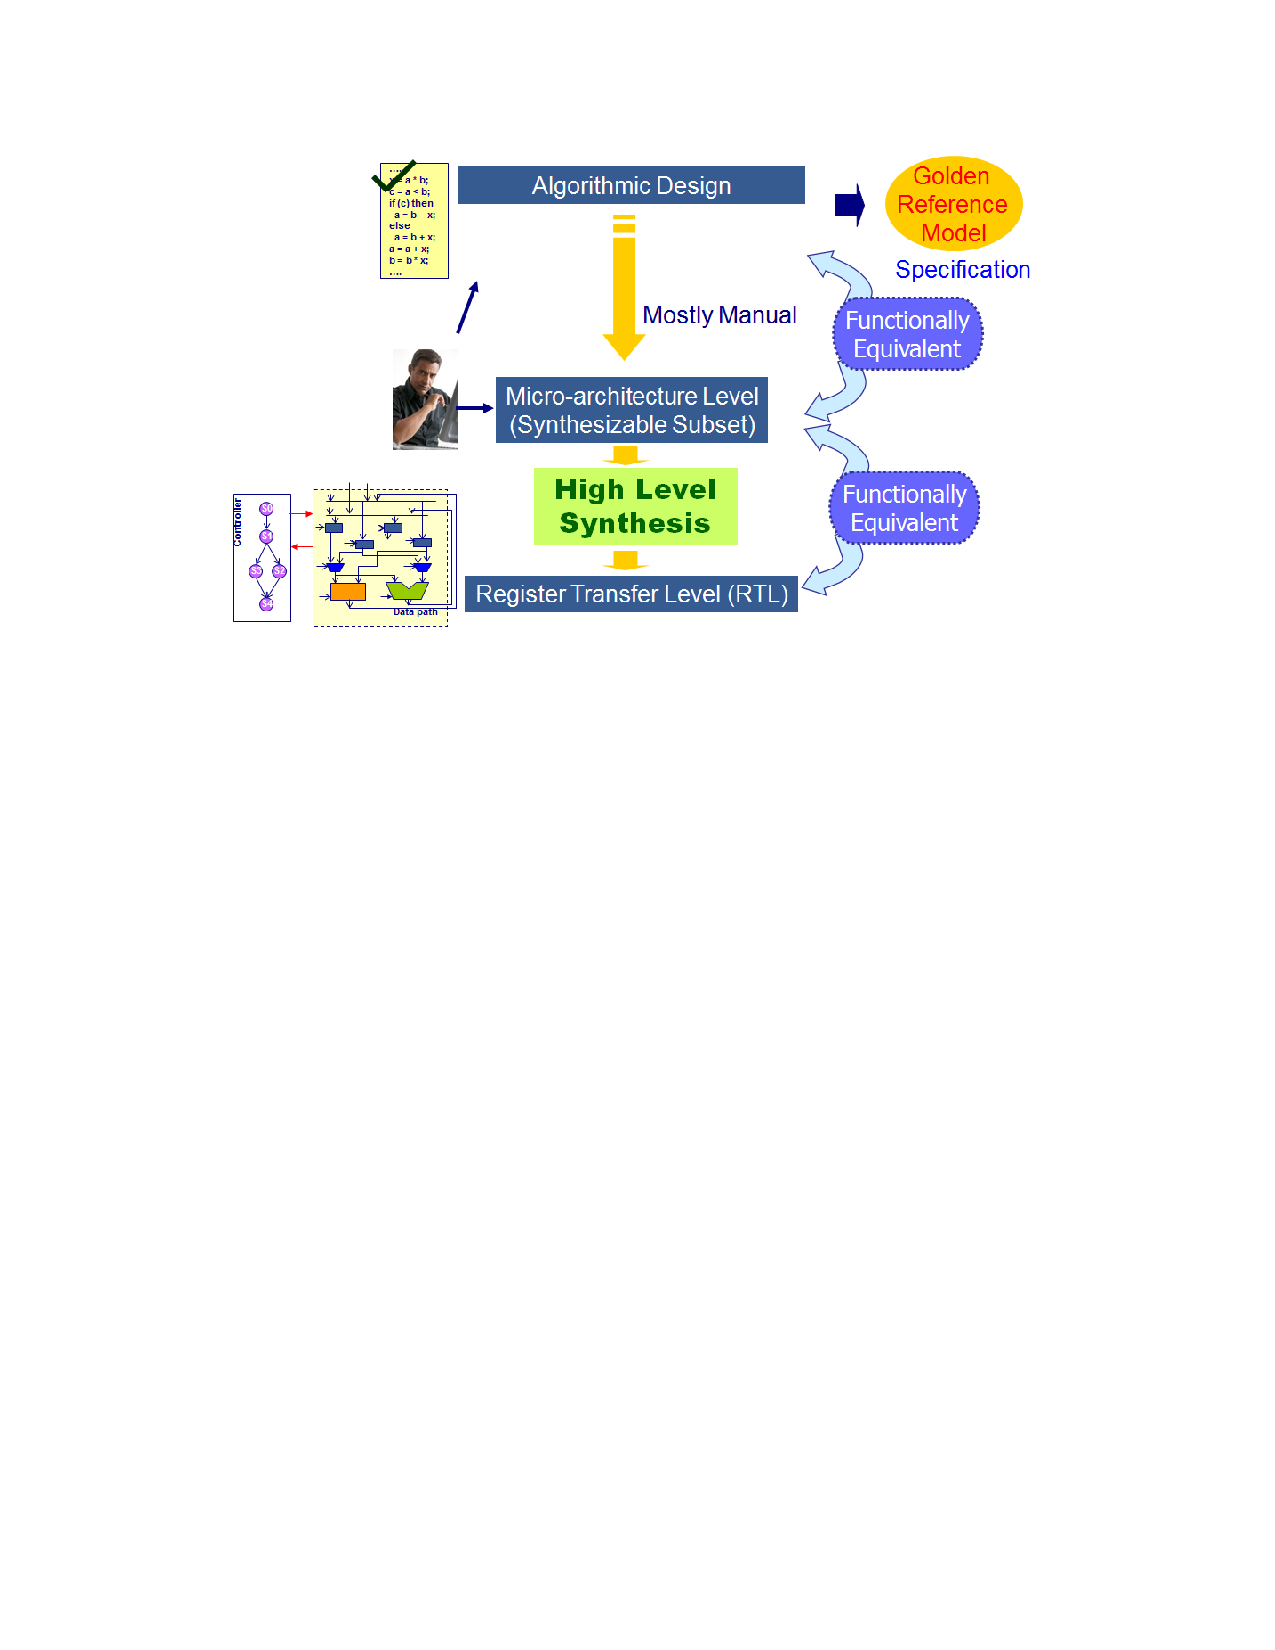
\includegraphics[width=0.7\tw]{verification-hls.pdf}
  \caption{\BF{Verification for High-Level Synthesis}}
  \label{fig-verification-hls}
\end{figure}



The accelerator subsystem includes a RISC-V RV64G Rocket core which
controls a binarized neural network (BNN) accelerator through the RoCC
interface. The BNN accelerator is a novel approach that goes far beyond
preliminary BNN implementations in the literature in that it binarizes
both the weights as well as the gradient calculations. The accelerator
subsystem uses high-level synthesis (HLS) motivating the need for a
different verification strategy from what was used in the processor
subsystem. HLS-design involves several incremental steps for bringing the
algorithm specified in the high-level program to low-level synthesized
RTL. Likewise, our verification methodology features tests at each stage
of the design flow to ensure that errors are not propagated in between
different stages of the model (see Figure~\ref{fig-verification-hls}).
Based on this principle, we first develop the algorithm in Python and
validate that it meets the desired design goals. This Python
implementation serves as the golden reference model. We then manually
transform this high-level representation into a lower-level untimed C++
implementation, and we use the golden reference model to verify the
functionality of the C++ implementation. We use high-level synthesis to
automatically transform the untimed C++ implementation into
cycle-accurate RTL, and we use the C++ implementation to verify the
functionality of the cycle-accurate RTL. We use a similar approach when
verifying our SystemC implementation.

% Our validation strategy consists of two components: (a) validation of
% the algorithm on a model of architecture by the system architect
% against a functional specification; (b) validation of design
% refinement; (c) formal verification of the translation and composition
% processes. We have implemented this strategy in a hierarchical fashion
% where individual IP written at behavioral levels with varying degrees
% of timing information are validated. Composition of validated designs
% is verified independently at a higher level of design hierarchy.

% For each validation task, we make distinction among three types of
% blocks: untimed, approximately timed and cycle-accurate descriptions.
% In the following sections, we describe the approach taken, followed by
% a discussion of the areas of improvement and potential for speeding up
% the validation process due to Compositional Synthesis approach devised
% by the CERTUS project.

% Untimed blocks consist of functional or imperative code blocks captured
% as functions, processes and modules. While functions/procedures
% represent well-defined algorithmic behaviors, processes represent
% non-terminating behaviors. Modules are characterized by structural
% interfaces that provide the basic unit of composition for the SOC
% design (see Figure below). Algorithmic design proceeds by a
% ``bottom-up'' development of the functional specification that is
% refined into an implementation in a programming language of choice.
% Architectural design proceeds by a ``top-down'' decomposition of
% functional blocks that is refined into an implementation. The two
% process run simultaneously providing ample opportunities for
% architecture-algorithm co-design by means of ``compositional glue''
% that enables simultaneous execution of heterogeneous functional blocks.

% Within the context of the CRAFT/CERTUS project, we have applied this
% co-design methodology in the design of a neural network accelerator
% that is composed with a predesigned RISC-V Rocketcore. There are two
% parts to a neural network design: determination of the matrix weights
% through an extensive ``training phase'' that is done offline. A trained
% network is implemented and used for a variety of ``recognition'' tasks
% (as one of the inferences that can be derived using a neural network.)
% We start with algorithmic description of a convolutional neural network
% (CNN) consisting of layers of processing. The CNN is typically
% described by means of data-flow graphs by algorithm designers and
% implemented using high-level libraries such as Theano Deep Learning
% Framework.

\paragraph{Validation of Algorithm}
The starting point of algorithmic design for the BNN is a manually
entered description of of the BNN in Python using Theano. We use the
MNIST and CFAR10 benchmarks images along with this high-level description
to validate that the algorithm achieves our design goals in terms of
classification accuracy and model size. We can also conduct preliminary
experiments to explore methods to improve the performance of the BNN
(e.g., spectral decomposition methods). We compared the performance of
BNN accelerator with the original floating-point convolutional neural
network on the CIFAR10 testing dataset, and we measured the image
classification error-rate to be $\approx$11.4\%. \fixme{I don't
  understand this. Is the error rate of the floating point CNN also
  11.4\%? Or is the BNN 11.4\% worse than the CNN? Rajesh, can you
  clarify?} This result is close to the state-of-the-art CIFAR10
classification result, while potentially having a higher computation
speed and smaller memory requirement. The result of algorithmic design
process is creation of a ``golden reference model'' against which all
subsequent validations take place.

% In the BNN acceleration algorithm implemented in CERTUS, we binarize
% both weights and activations of the network. This reduces the size of
% parameters and changes the arithmetic operations into bitwise
% operations thus accelerating the inference algorithm. The
% implementation of BNN includes reading the Python-trained BNN model
% parameters to the BNN network and classification of the CIFAR10 image
% dataset. The network is composed to six convolutional layers with 3x3
% filters, three 2x2 padding layers and three fully-connected layers.

% \BF{Architectural Design and Implementation}

% The entire process of binarization of the CNN algorithm is conducted in
% Python. Once we have converged on the quality of binarized CNN results,
% the SOC accelerator design process starts. We start with a reference
% model in Python/Theano where design refinement into implementation
% compares results of layer-by-layer computations on image benchmarks
% against the reference implementation. There is no approximation in the
% feedforward stage and hence this comparison can be made to exact
% numerical values. Indeed, the process of binarization in CNN actually
% assists in validation since the layer computation results can now be
% compared to be bitwise identical to the reference implementation.

% As a part of algorithm design, the BNN network models were trained in
% Theano in Python. We trained various models for different settings:
% original BNN, reduced BNN, BNN without bias, and BNN with non-zero
% padding values. These various algorithmic choices were analyzed for
% performance and model size. The algorithm design group handed off
% reference Python code and all trained models to the SOC accelerator
% design team for implementation in hardware.

% For BNN verification in algorithm level, we compared the output values
% of C program with Python program for each layer in the BNN network.
% These have the same values throughout the network and their final
% output are also identical. So the BNN in C program is in accordance
% with the theoretical BNN network we designed and also the BNN model we
% implemented in Python.

% For Hardware implementation verification, we provided the C and Python
% programs and model parameters, along with the expected output of
% CIFAR10 dataset to accelerator architectural design group at Cornell.
% The output of the Python program provides the golden reference model
% that is used in validating the architectural implementation of BNN
% hardware.

\paragraph{Testing the Manually Written C++ Implementation}
We manually transform the high-level Python algorithm into a lower-level
C++ implementation. We use standard software testing practices to verify
that the C++ implementation matches the golden reference model. Our
simplest test ensures that the C++ model performs 3D convolution and
binarization correctly on randomly generated feature maps and conv
filters. The model reads in the random data and produces a single output
binary feature map, which is then compared against the output of a golden
reference model. The random test provides a small initial test, but it
only tests a single output image. Furthermore, it does not test the input
conv layer, the dense layers, or max pooling.

Further verification compares the BNN C++ model against the golden
reference model on a layer-by-layer basis. Intermediate feature maps from
the golden reference model program were first dumped to disk. The
testbench then verifies a single layer by sending in the dumped input
feature maps and comparing the output with the dumped output feature
maps. We have developed tests for all three layer types (i.e., input
conv, binary conv, and dense), and these tests verify the layers in
isolation. Note that due to hardware model optimizations (e.g.,
fixed-point) there will be some discrepancy in the results, but the
expected rate of incorrect bits on a single layer is less than 2\%.

We also use end-to-end tests to verify the entire BNN by sending in
CIFAR-10 test images and comparing the output class labels to the golden
reference model. These tests can operate on a single image or a batch of
images. Again, the hardware model optimizations mean that the accuracy
over thousands of images may not exactly match the golden reference
model. We consider the implementation to be correct if the accuracy
difference is negligible (less than 0.5\%).

\paragraph{Testing the RTL Generated Automatically Through C++ HLS}
Our verification flow benefits from advances in co-simulation which
allows direct reuse of the original C++ software testbenches to drive RTL
simulation of the HLS-generated accelerator. Co-simulation significantly
alleviates verification effort by avoiding the need for timing-consuming
manual creation of RTL testbenches. Because RTL simulation is slow, we
only run the smaller test cases. We use FPGA emulation to run the
end-to-end tests. FPGA emulation tests the accuracy of the BNN in real
hardware, and ensures the accuracy matches that of the C++ model.

\paragraph{Testing the SystemC Implementation}
Our ASIC HLS flow requires SystemC for design entry. We are mostly able
to reuse our C++ implementation and simply add SystemC-specific
constructs and interfaces. This also enables reusing many of the
testbenches developed for verifying the C++ model. Similar to the C++
testing flow, we performed SystemC (behavioral) simulation to verify the
correctness of the SystemC functional specifications compared against the
golden reference model.

\paragraph{Testing the RTL Generated Automatically Through SystemC HLS}
We again leverage recent advances in co-simulation to facilitate
productive verification of the RTL generated through SystemC HLS. A major
roadblock in our design flow stemmed from bugs inherent in the
SystemC-to-RTL synthesis process. We were experiencing mismatches between
results from behavioral simulation and RTL simulation which are due to
bugs in the SystemC HLS tool. Our strategy relied on using
``synthesizable print statements'' in SystemC. Essentially, we were able
to use print statements to output variables during SystemC simulation,
and these print statements were synthesized into similar print statements
in the generated Verilog RTL to output the same variables during Verilog
RTL simulation. We wrote custom tools to compare these trace outputs to
localize mismatches, and we created unit test cases that specifically
target these mismatches. This process enabled us to gradually refine our
SystemC implementation to avoid simulation/synthesis mismatches.

\paragraph{Testing the Rocket+Accelerator RTL}
Once we have verified the Rocket core RTL in isolation and the generated
RTL for the BNN accelerator in isolation, we perform integration testing
to verify the composition of the Rocket RTL and BNN accelerator RTL. This
testing proceeds in three steps.

The first step involves writing small self-checking assembly test
programs. For example, we have written minimal assembly tests that use
the RISC-V custom instructions to simply write and read a special testing
register within the BNN accelerator. This enables verifying the Rocket
core is correctly executing the custom instructions, that these custom
instructions are being turned into correct RoCC messages, and that the
accelerator is able to process these RoCC messages. Other minimal
assembly tests are able to verify very small parts of the BNN accelerator
in isolation.

The second step involves writing small C test programs which are similar
in spirit to the layer and end-to-end tests used in testing the BNN
accelerator in isolation. Of course, the difference is that these small C
test programs are cross-compiled and execute on the actual Rocket core.
These small C test programs use the bare-metal software stack, meaning
they do not use the memory management unit nor any system calls. This
enables testing larger parts of the BNN accelerator and also the
interaction between the Rocket core and the BNN accelerator through the
memory system.

The third step is to execute these small C test programs on the
proxy-kernel software stack, and to write more complex C test programs
that use memory management unit and/or system calls. This enables testing
more realistic workloads, but also enables verifying the interaction
between the Rocket core, the BNN accelerator, and the memory management
unit. In fact, we identified a critical issue through this final
integration testing. All RoCC accelerators in the version of the Rocket
core used in this project use physical addresses and thus never causes
page faults. The Berkeley proxy-kernel software-stack relies on
page faults to implement lazy program loading and dynamic memory
initialization. Our work-around is to make sure that any page which the
accelerator accesses is first touched by the Rocket core to ensure
corresponding page is already loaded/initialized in physical memory. We are working on modifying the proxy-kernel to support physical-memory modes.

